\section{R / Hive (07.06.2018)}
\begin{itemize}
\item[-] Suchen Sie sich einen für Sie interessanten Bereich aus bspw. Marktforschung, soziale Netzwerke, Wetterstationen, Gesundheitswesen, Natur und Sozialwissenschaften, etc.
\item[-] Erzeugen Sie für Ihr Beispiel zwei Hive Tabellen
\item[-] Füllen Sie die Tabellen mit einigen Testdaten (LOAD DATA, Insert).
\item[-] Bauen Sie eine R Verbindung zur HIVE auf.
\item[-] Analysieren Sie die Daten
\end{itemize}
\subsection*{Kurzdarstellung der Aufgabenstellung}
Mittels dem Anlegen von zwei Tabellen in HIVE und dem anschließenden Bearbeiten/Analysieren mit R soll die das Zusammenspiel von relevanter Software für BigData geübt/demonstriert werden.
\subsection*{Lösung}
\subsubsection*{HIVE}
\begin{itemize}
\item[-] Ordner in /usr/tmp/hive/ anlegen
\item[-] Datensets „hotels.csv“ und „autos.csv“  in /usr/tmp/hive/ legen
\item[-] HIVE über den Terminal in Oracle VM4.9:

\begin{lstlisting}
HIVE
\end{lstlisting}

\item[-] Separate Datenbank im HIVE anlegen, falls keine namentlich identische existiert:
\begin{lstlisting}
CREATE DATABASE IF NOT EXISTS diim18;
\end{lstlisting}

\item[-] Tabelle „hotels“ anlegen mit folgendem Befehl:
\begin{lstlisting}
Create TABLE hotels(gewinn FLOAT, preisInMio FLOAT,qm FLOAT,stadt String) ROW Format DELIMITED FIELDS Terminated by ',' Lines terminated by '\n';
\end{lstlisting}

\item[-] Tabelle „autos“ anlegen mit folgendem Befehl:
\begin{lstlisting}
Create TABLE autos(preis FLOAT, registrierungJahr INT,ps FLOAT,km INT,  modell String, kraftstoff STRING, name STRING) ROW Format DELIMITED FIELDS      Terminated by ',' Lines terminated by '\n';
\end{lstlisting}

\item[-] Daten aus hotels.csv in HIVE Tabelle hotels laden:
\begin{lstlisting}
LOAD DATA LOCAL INPATH '/usr/tmp/hive/hotels/hotels.csv' Overwrite INTO Table hotels;
\end{lstlisting}

\item[-] Daten aus hotels.csv in HIVE Tabelle hotels laden:
\begin{lstlisting}
LOAD DATA LOCAL INPATH '/usr/tmp/hive/autos/autos.csv' Overwrite INTO Table autos;
\end{lstlisting}
\item[-] Ausgabe der angelegten Tabellen.(\autoref{fig:hive1})
\begin{figure}[!htb]
        \begin{minipage}{1\textwidth}
                \centering
                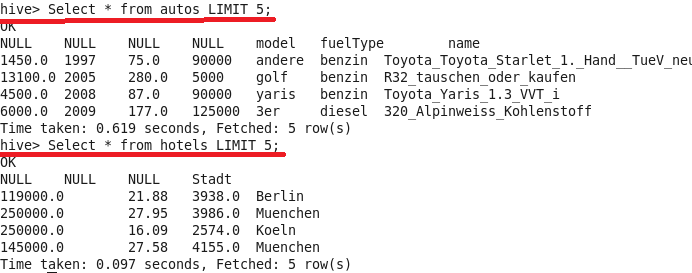
\includegraphics[width=0.90\textwidth]{pics/HIVE.png}\par\vspace{0cm}
                \caption{Ausgabe Tabellen}
                \label{fig:hive1}
        \end{minipage}
\end{figure}
Die Daten können nun mit SQL Statements betrachtet und manipuliert werden

\subsubsection*{R}
\item[-]Starten von R durch Eingabe in den terminal auf der Oracle 4.9 VM:
\begin{lstlisting}
R
\end{lstlisting}

\item[-] Installieren des RJDBC packages:
\begin{lstlisting}
install.packages("RJDBC",dep=TRUE)
\end{lstlisting}

\item[-] Aufrufen des RJDBC packages:
\begin{lstlisting}
library("RJDBC")
\end{lstlisting}

\item[-] Driver auf variable in R zur Verwendung zuweisen:
\begin{lstlisting}
drv <-JDBC("org.apache.hive.jdbc.HiveDriver","/usr/lib/hive/lib         /hive-jdbc.jar")
\end{lstlisting}

\item[-] Connection Type hinzufügen:

\begin{lstlisting}
library("ORCH")
ore.connect(type="HIVE")
ore.sync()
\end{lstlisting}

\item[-] Verbindung zu R aufbauen
\begin{lstlisting}
conn <- dbConnect(drv, "jdbc:hive2://localhost:10000/diim18", "", "")
\end{lstlisting}

\item[-] Inhalt der Tabelle autos im Hive auf die Variable autos in R zuweisen:
\begin{lstlisting}
autos <- dbGetQuery(conn, "Select * from autos")
\end{lstlisting}

\item[-] Lineares Regressionsmodell (lRm) erstellen: autos.preis = a * autos.km + b
\begin{lstlisting}
model <-lm(autos.preis~autos.km, data = autos)
\end{lstlisting}

\item[-] Modell Zusammenfassung ausgeben lassen (\autoref{fig:hive2}):
\begin{figure}[!htb]
        \begin{minipage}{1\textwidth}
                \centering
                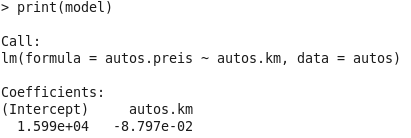
\includegraphics[width=0.60\textwidth]{pics/autos_model_1.png}\par\vspace{0cm}
                \caption{Ausgabe: model}
                \label{fig:hive2}
        \end{minipage}
\end{figure}


\item[-] Erstellen einer neuen Spalte in Autos die den Preis auf Basis des lRm:
\begin{lstlisting}
autos$predicted_1 <- predict(model, autos)
\end{lstlisting}

\item[-] multiples Rm (mRm) erstellen: autos.preis = a * autos.km + b * autos.ps + b
\begin{lstlisting}
model <-lm(autos.preis~autos.km+autos.ps, data = autos)
\end{lstlisting}

\item[-] Modell Zusammenfassung ausgeben lassen (\autoref{fig:hive3}):
\begin{figure}[!htb]
        \begin{minipage}{1\textwidth}
                \centering
                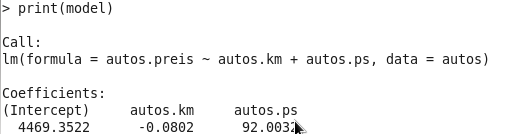
\includegraphics[width=0.60\textwidth]{pics/autos_model_2.png}\par\vspace{0cm}
                \caption{Ausgabe: model}
                \label{fig:hive3}
        \end{minipage}
\end{figure}


\item[-] Erstellen einer neuen Spalte in Autos die den Preis auf Basis des mRm (\autoref{fig:hive4})
\begin{lstlisting}
autos$predicted_2 <- predict(model, autos)
print(model)
head(autos)
\end{lstlisting}
\begin{figure}[!htb]
        \begin{minipage}{1\textwidth}
                \centering
                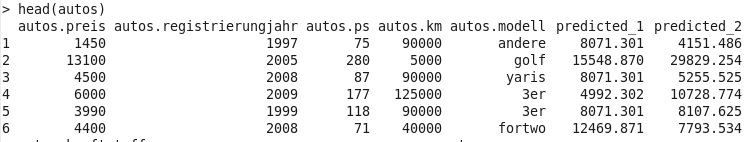
\includegraphics[width=0.70\textwidth]{pics/autos_head.png}\par\vspace{0cm}
                \caption{Ausgabe: autos}
                \label{fig:hive4}
        \end{minipage}
\end{figure}
\item[-] Inhalt der Tabelle autos im Hive auf die Variable autos in R zuweisen:
\begin{lstlisting}
hotels <- dbGetQuery(conn, "Select * from hotels")
\end{lstlisting}

\item[-] Lineares Regressionsmodell (lRm) erstellen: hotels.preisinmio = a * hotels.gewinn + b * hotels.qm
\begin{lstlisting}
model <-lm(hotels.preisinmio~hotels.gewinn+hotels.qm, data = hotels)
\end{lstlisting}

\item[-] Erstellen einer neuen Spalte in Autos die den Preis auf Basis des lRm:
\begin{lstlisting}
hotels$predicted_1 <- predict(model, hotels)
\end{lstlisting}

\item[-] Modell Zusammenfassung ausgeben lassen (\autoref{fig:hive5}):
\begin{figure}[!htb]
        \begin{minipage}{1\textwidth}
                \centering
                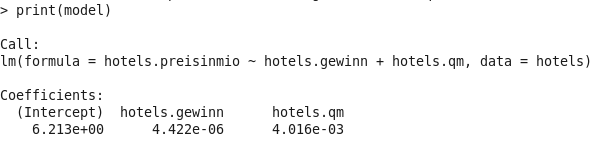
\includegraphics[width=0.70\textwidth]{pics/Hotels_model_1.png}\par\vspace{0cm}
                \caption{Ausgabe: hotels}
                \label{fig:hive5}
        \end{minipage}
\end{figure}


\item[-] multiples Rm (mRm) erstellen: hotels.preisinmio = a * hotels.gewinn + b * hotels.qm + c * hotels.stadt
\begin{lstlisting}
model <-lm(hotels.preisinmio~hotels.gewinn+hotels.qm+hotels.stadt, data = hotels)
\end{lstlisting}

\item[-] Modell Zusammenfassung ausgeben lassen (\autoref{fig:hive6})
\begin{figure}[!htb]
        \begin{minipage}{1\textwidth}
                \centering
                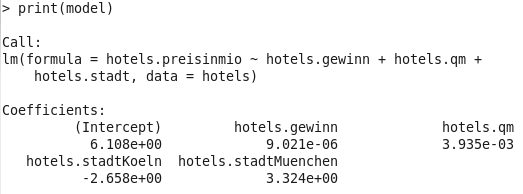
\includegraphics[width=0.70\textwidth]{pics/Hotels_model_2.png}\par\vspace{0cm}
                \caption{Ausgabe: hotels}
                \label{fig:hive6}
        \end{minipage}
\end{figure}
\item[-] Erstellen einer neuen Spalte in Autos die den Preis auf Basis des mRm (\autoref{fig:hive7}: 
\begin{lstlisting}
hotels$predicted\_2 <- predict(model, hotels)
\end{lstlisting}
\begin{figure}[!htb]
        \begin{minipage}{1\textwidth}
                \centering
                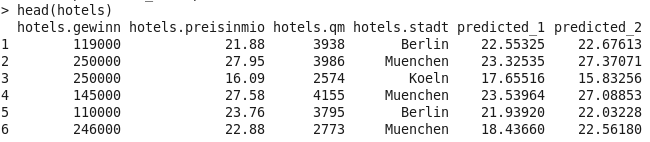
\includegraphics[width=0.70\textwidth]{pics/hotels_head.png}\par\vspace{0cm}
                \caption{Ausgabe: hotels}
                \label{fig:hive7}
        \end{minipage}
\end{figure}
\end{itemize}

\subsection*{Aufteilung der Aufgaben im Team}
\subsection*{Darstellung der benutzen Werkzeuge und Systeme}
\subsubsection*{Entwurfswerkzeug}
- HIVE 

\subsubsection*{Entwicklungsumgebung}
- R

